\documentclass[a4paper]{article}

\usepackage[UTF8]{ctex}
\usepackage[a4paper,margin=1in]{geometry}
\usepackage{graphicx}
\usepackage{float}
\usepackage{listings}
\usepackage{longtable}
\usepackage{booktabs}
\usepackage{hyperref}
\usepackage{fancyhdr}
\usepackage{lastpage}
\usepackage{color}
\usepackage{indentfirst}        % 首段缩进
\setlength{\parindent}{2em}     % 缩进2字符
\usepackage{zhnumber}           % 中文编号
\usepackage[dvipsnames]{xcolor}
\usepackage{amsmath}
\newcommand{\college}{中山大学计算机学院}
\newcommand{\projname}{机器学习与数据挖掘|作业二}
\newcommand{\reporttitle}{evaluation metrics}
\newcommand{\stuno}{23336179}
\newcommand{\authorname}{马福泉}
\newcommand{\major}{计算机科学与技术}
\newcommand{\adviser}{梁上松}
\newcommand{\startdate}{2025年9月28日}
\newcommand{\labenddate}{2025年9月29日}
\newcommand{\labroom}{c206}

\pagestyle{fancy} % 使用 fancyhdr 风格
\fancyhf{}      % 清空默认的页眉页脚

% 设置页眉
\fancyhead[L]{\kaishu \projname}      % 左侧页眉显示项目名称
\fancyhead[C]{\kaishu \reporttitle}    % 中间页眉显示报告标题
\fancyhead[R]{\kaishu \authorname} % 右侧页眉显示作者姓名

% 设置页脚
\fancyfoot[C]{第 \thepage 页，共 \pageref{LastPage} 页} % 中间页脚显示页码

% 去除页眉页脚与正文之间的分隔线
\renewcommand{\headrulewidth}{0.4pt}
\renewcommand{\footrulewidth}{0pt}

% 设置文档背景颜色
\definecolor{mybgcolor}{RGB}{0, 0, 0} % 定义背景颜色
\definecolor{NavyBlue}{RGB}{0,0,128} % 添加颜色定义
% \pagecolor{mybgcolor} % 设置背景颜色

% listing 配置rust
% \lstdefinelanguage{Rust}{
%   keywords={fn, let, mut, struct, enum, impl, pub, use, mod, trait, where},
%   keywordstyle=\color{NavyBlue},
%   comment=[l]{//},
%   commentstyle=\color{gray},
% }
% \lstset{language=Rust}

\begin{document}

% 封面
\begin{titlepage}
    \centering
    

    
\includegraphics[width=10cm]{img/SYSULogo.png}

    \vspace{1em}
    %{\Large \college \par}
    \vspace{1em}
    {\Large \kaishu \projname \par}
    \vspace{3em}

    

    
    {\fontsize{40pt}{42pt}\kaishu \selectfont \boldmath \reporttitle\par}
    \vspace*{\fill}

    \begin{center}
    {\Large
    \makebox[5em][s]{学号}:\underline{\makebox[15em][c]{\kaishu \stuno}}\\[1em]
    \makebox[5em][s]{姓名}:\underline{\makebox[15em][c]{\kaishu \authorname}}\\[1em]
    \makebox[5em][s]{专业}:\underline{\makebox[15em][c]{\kaishu \major}}\\[1em]
    \makebox[5em][s]{课程教师}:\underline{\makebox[15em][c]{\kaishu \adviser}}\\[1em]
    \makebox[5em][s]{起始日期}:\underline{\makebox[15em][c]{\kaishu \startdate}}\\[1em]
    \makebox[5em][s]{结束日期}:\underline{\makebox[15em][c]{\kaishu \labenddate}}\\[1em]
    \makebox[5em][s]{实验地点}:\underline{\makebox[15em][c]{\kaishu \labroom}}
    }
    \end{center}

    \vspace*{\fill}
\end{titlepage}

% 目录
\tableofcontents
\newpage

% ===================== 作业内容 =====================



\section{练习1: 基于排名的评估指标，MAP@K，MRR@K}

假设您有三个查询，系统针对这三个查询的排名结果如下：

排名1（响应查询\#1）：d1, d2, d3, d4, d5, d6, d7, d8, d9, d10。这里只有d1, d3, d4, d6, d7和d10是相关的（相关性是二元的，即相关为1，不相关为0）。

排名2（响应查询\#2）：d3, d8, d7, d1, d2, d4, d5, d9, d10, d6。这里只有d8和d9是相关的。

排名3（响应查询\#3）：d7, d6, d5, d3, d2, d1, d9, d10, d4, d8。这里只有d5, d9和d8是相关的。

请回答以下问题：

(a) 计算这些指标的分数：每个查询的AP@5（平均精度@5）、AP@10；每个查询的RR@5（倒数排名分数@5）、RR@10。

(b) 计算这些指标的分数：该系统的MAP@5（平均精度均值@5）、MAP@10、MRR@5（平均倒数排名分数@5）、MRR@10。

\subsection{计算过程和结果}

\begin{figure}[H]
    \centering
    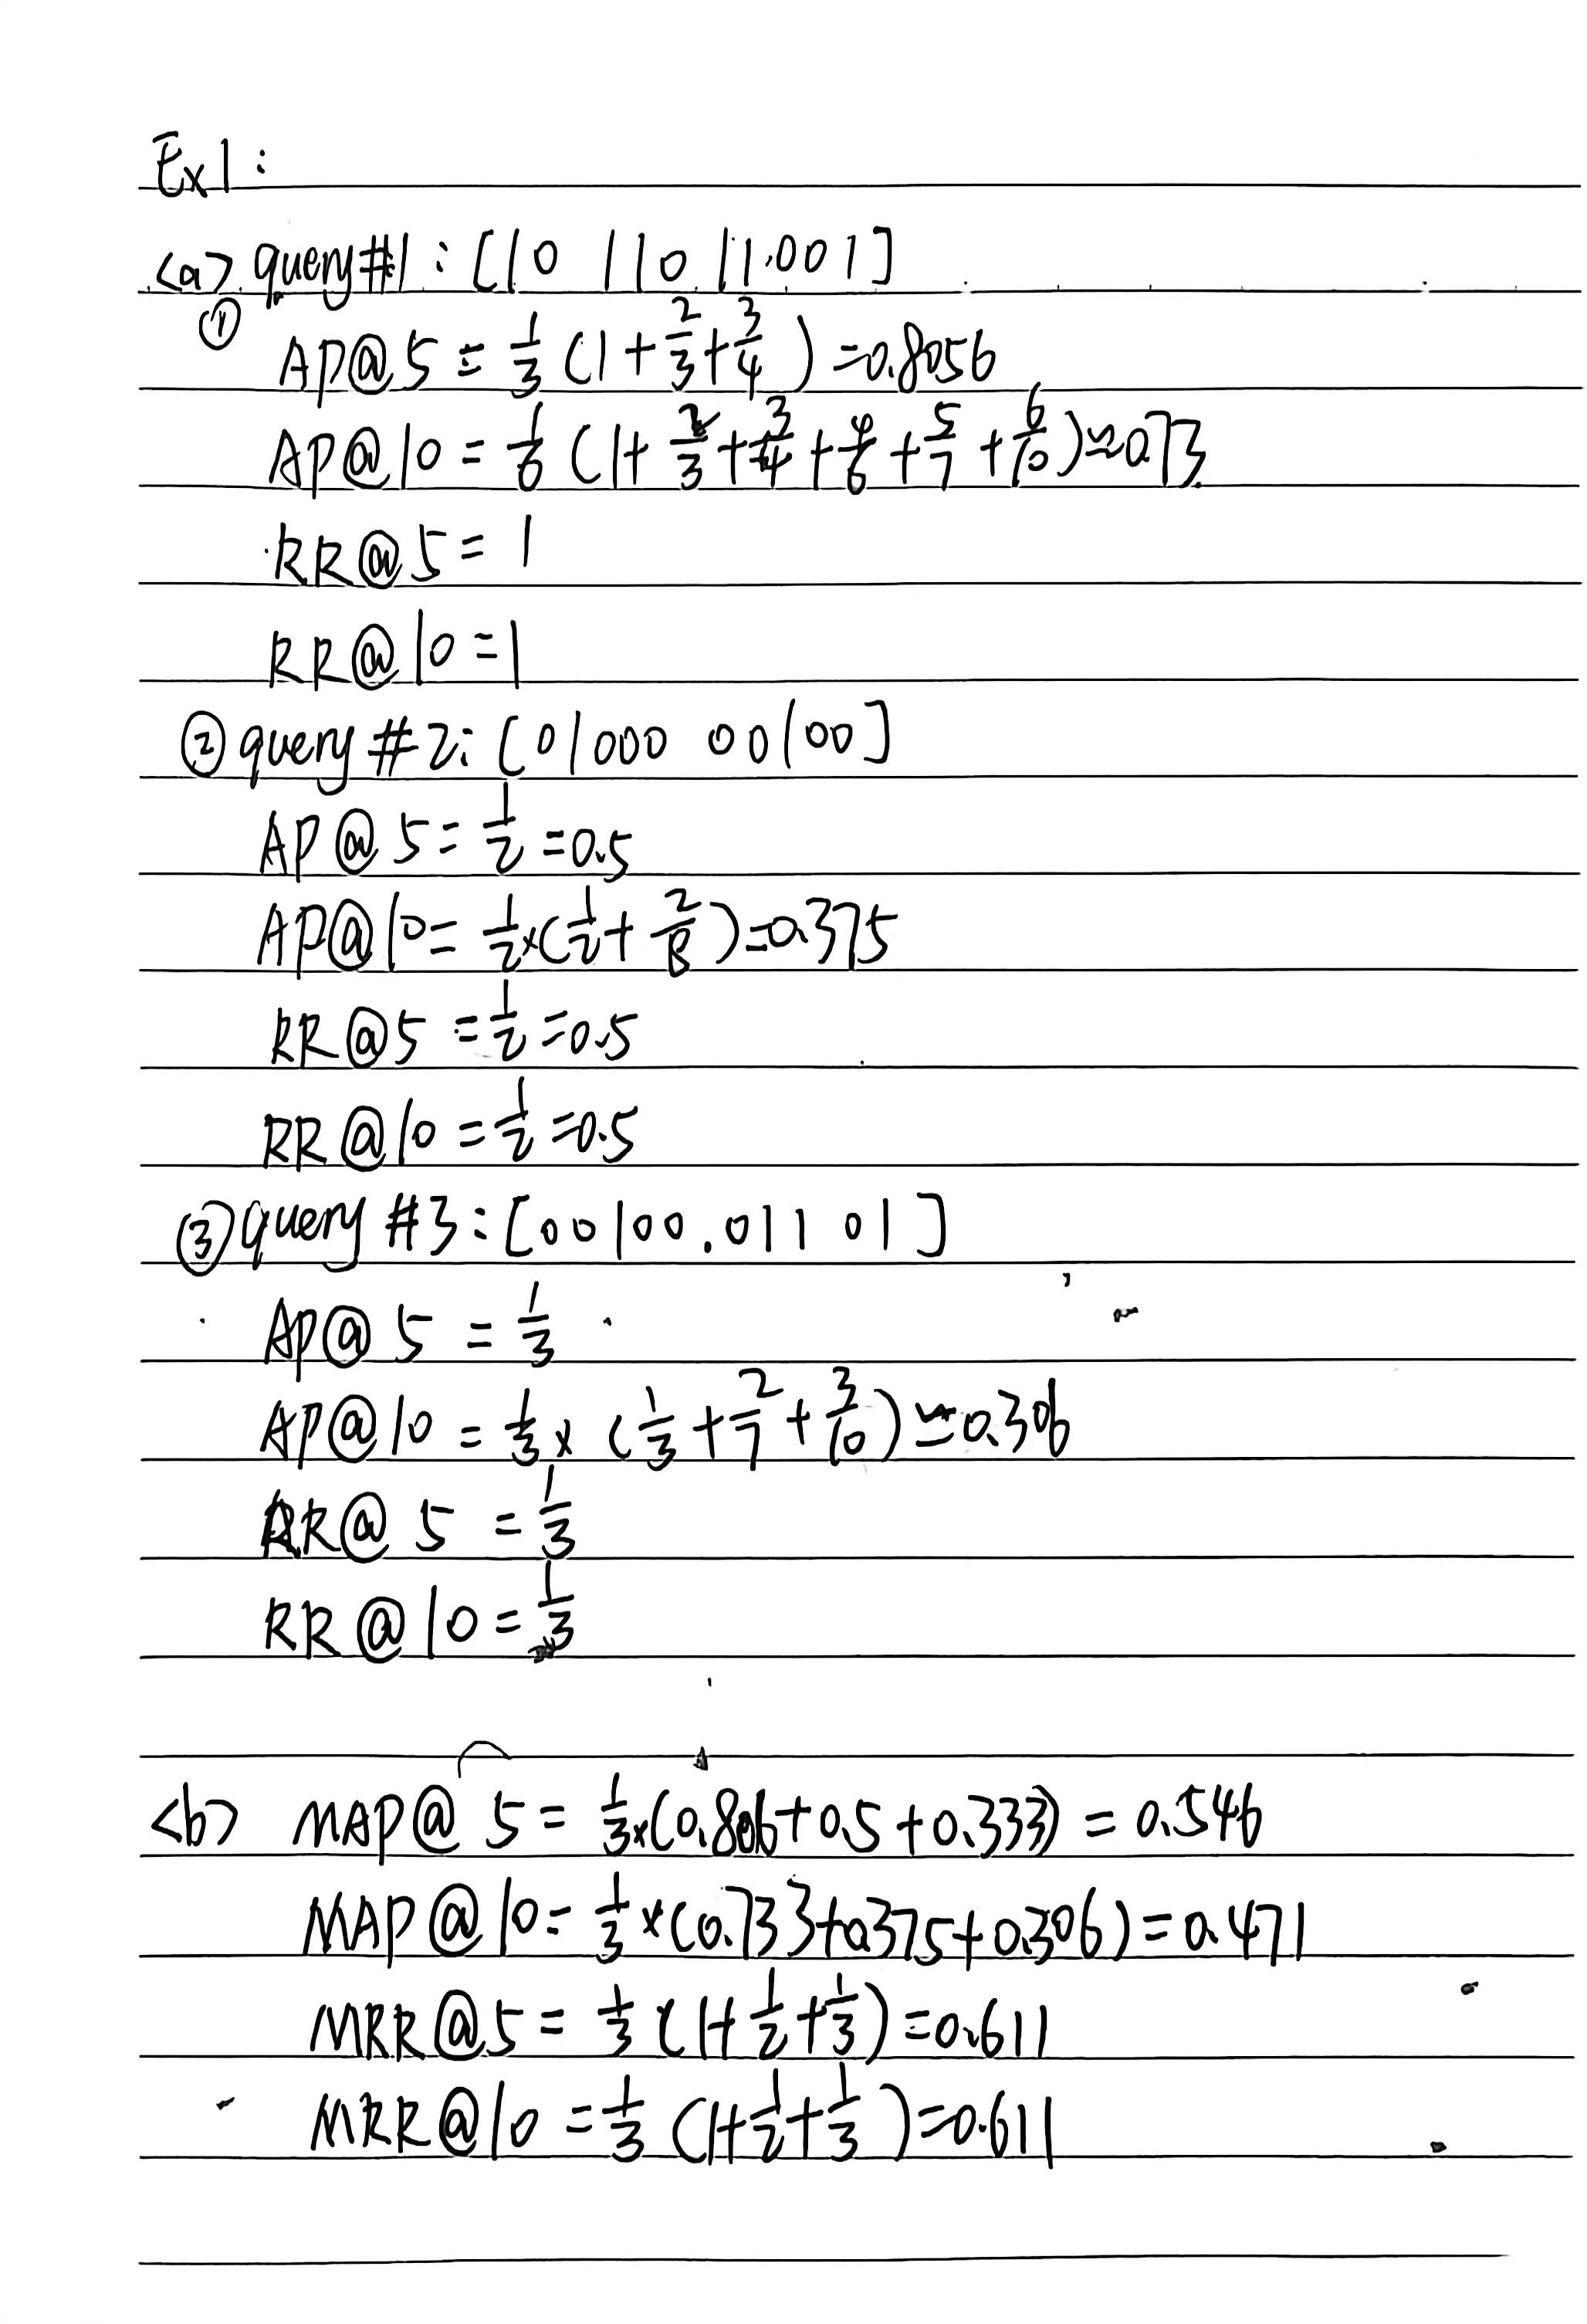
\includegraphics[width=\textwidth]{img/ex1_result.png}
    \caption{练习1计算过程}
    \label{fig:ex1_result}
\end{figure}


\section{练习2: 基于排名的评估指标，Precision@K，Recall@K，NDCG@K}

假设给定查询的以下排名（仅显示结果1-10）；见表1。"rank"列给出了文档的排名。"docID"列给出了与该排名关联的文档ID。"graded relevance"列给出了与文档相关的相关性等级（4=完美，3=优秀，2=良好，1=一般，0=差）。"binary relevance"列提供了两个相关性值（1=相关，0=不相关）。假设相关性等级为"一般"或更好的任何内容都是相关的，相关性等级为"差"的任何内容都是不相关的。

同时，假设此查询只有7个相关性等级为一般或更好的文档。这些文档都在给定排名的前10名中。

请回答以下问题。P@K（精度@K）、R@K（召回率@K）和平均精度（AP）假设二元相关性。对于这些指标，请使用"binary relevance"列。DCG和NDCG假设分级相关性。对于这些指标，请使用"graded relevance"列。

\begin{figure}[H]
    \centering
    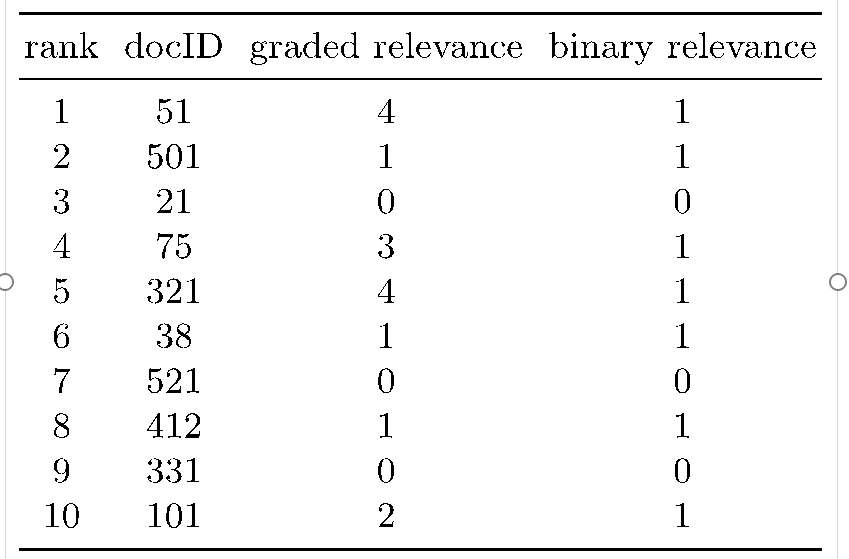
\includegraphics[width=\textwidth]{img/table1.png}
    \caption{表1 系统响应查询的前10名排名结果。}
    \label{fig:table1}
\end{figure}


(a) 计算P@5和P@10。

(b) 计算R@5和R@10。

(c) 提供一个使P@5最大化的此查询排名示例。

(d) 提供一个使P@10最大化的此查询排名示例。

(e) 提供一个使R@5最大化的此查询排名示例。

(f) 提供一个使R@10最大化的此查询排名示例。

(g) 您有理由相信此系统的用户将希望检查给定查询的每个相关文档。换句话说，您有理由相信用户希望完美的召回率。您希望基于P@K进行评估。在这种情况下，是否有设置K值的查询特定方法特别合适？是什么？（提示：有一个叫做R-Precision的评估指标，我们在讲座中没有讨论。您的答案应该与R-Precision相关。Wikipedia/Google可能会有帮助。）

(h) 计算平均精度（AP）。AP和MAP（平均精度均值）之间有什么区别？

(i) 提供一个使平均精度（AP）最大化的此查询排名示例。

(j) 计算DCG5（即第5位的折扣累计增益）。

(k) NDCG5由以下公式给出：
$$NDCG5 = \frac{DCG5}{IDCG5}$$

其中IDCG5是与此查询相关的理想前5名排名的DCG5。计算NDCG5需要三个步骤：
\begin{enumerate}
    \item[(i)] 与此查询相关的理想前5名排名是什么（注意查询有2个完美文档，1个优秀文档，1个良好文档，3个一般文档，其余文档都是差的）？
    \item[(ii)] IDCG5是与理想排名相关的DCG5。计算IDCG5。（提示：为您在部分(i)中提出的排名计算DCG5。）
    \item[(iii)] 使用上面的公式计算NDCG5。
\end{enumerate}

(l) 是否还有其他评估指标可用于评估表中排名的性能？这些指标获得的评估分数是多少？

\begin{figure}[H]
    \centering
    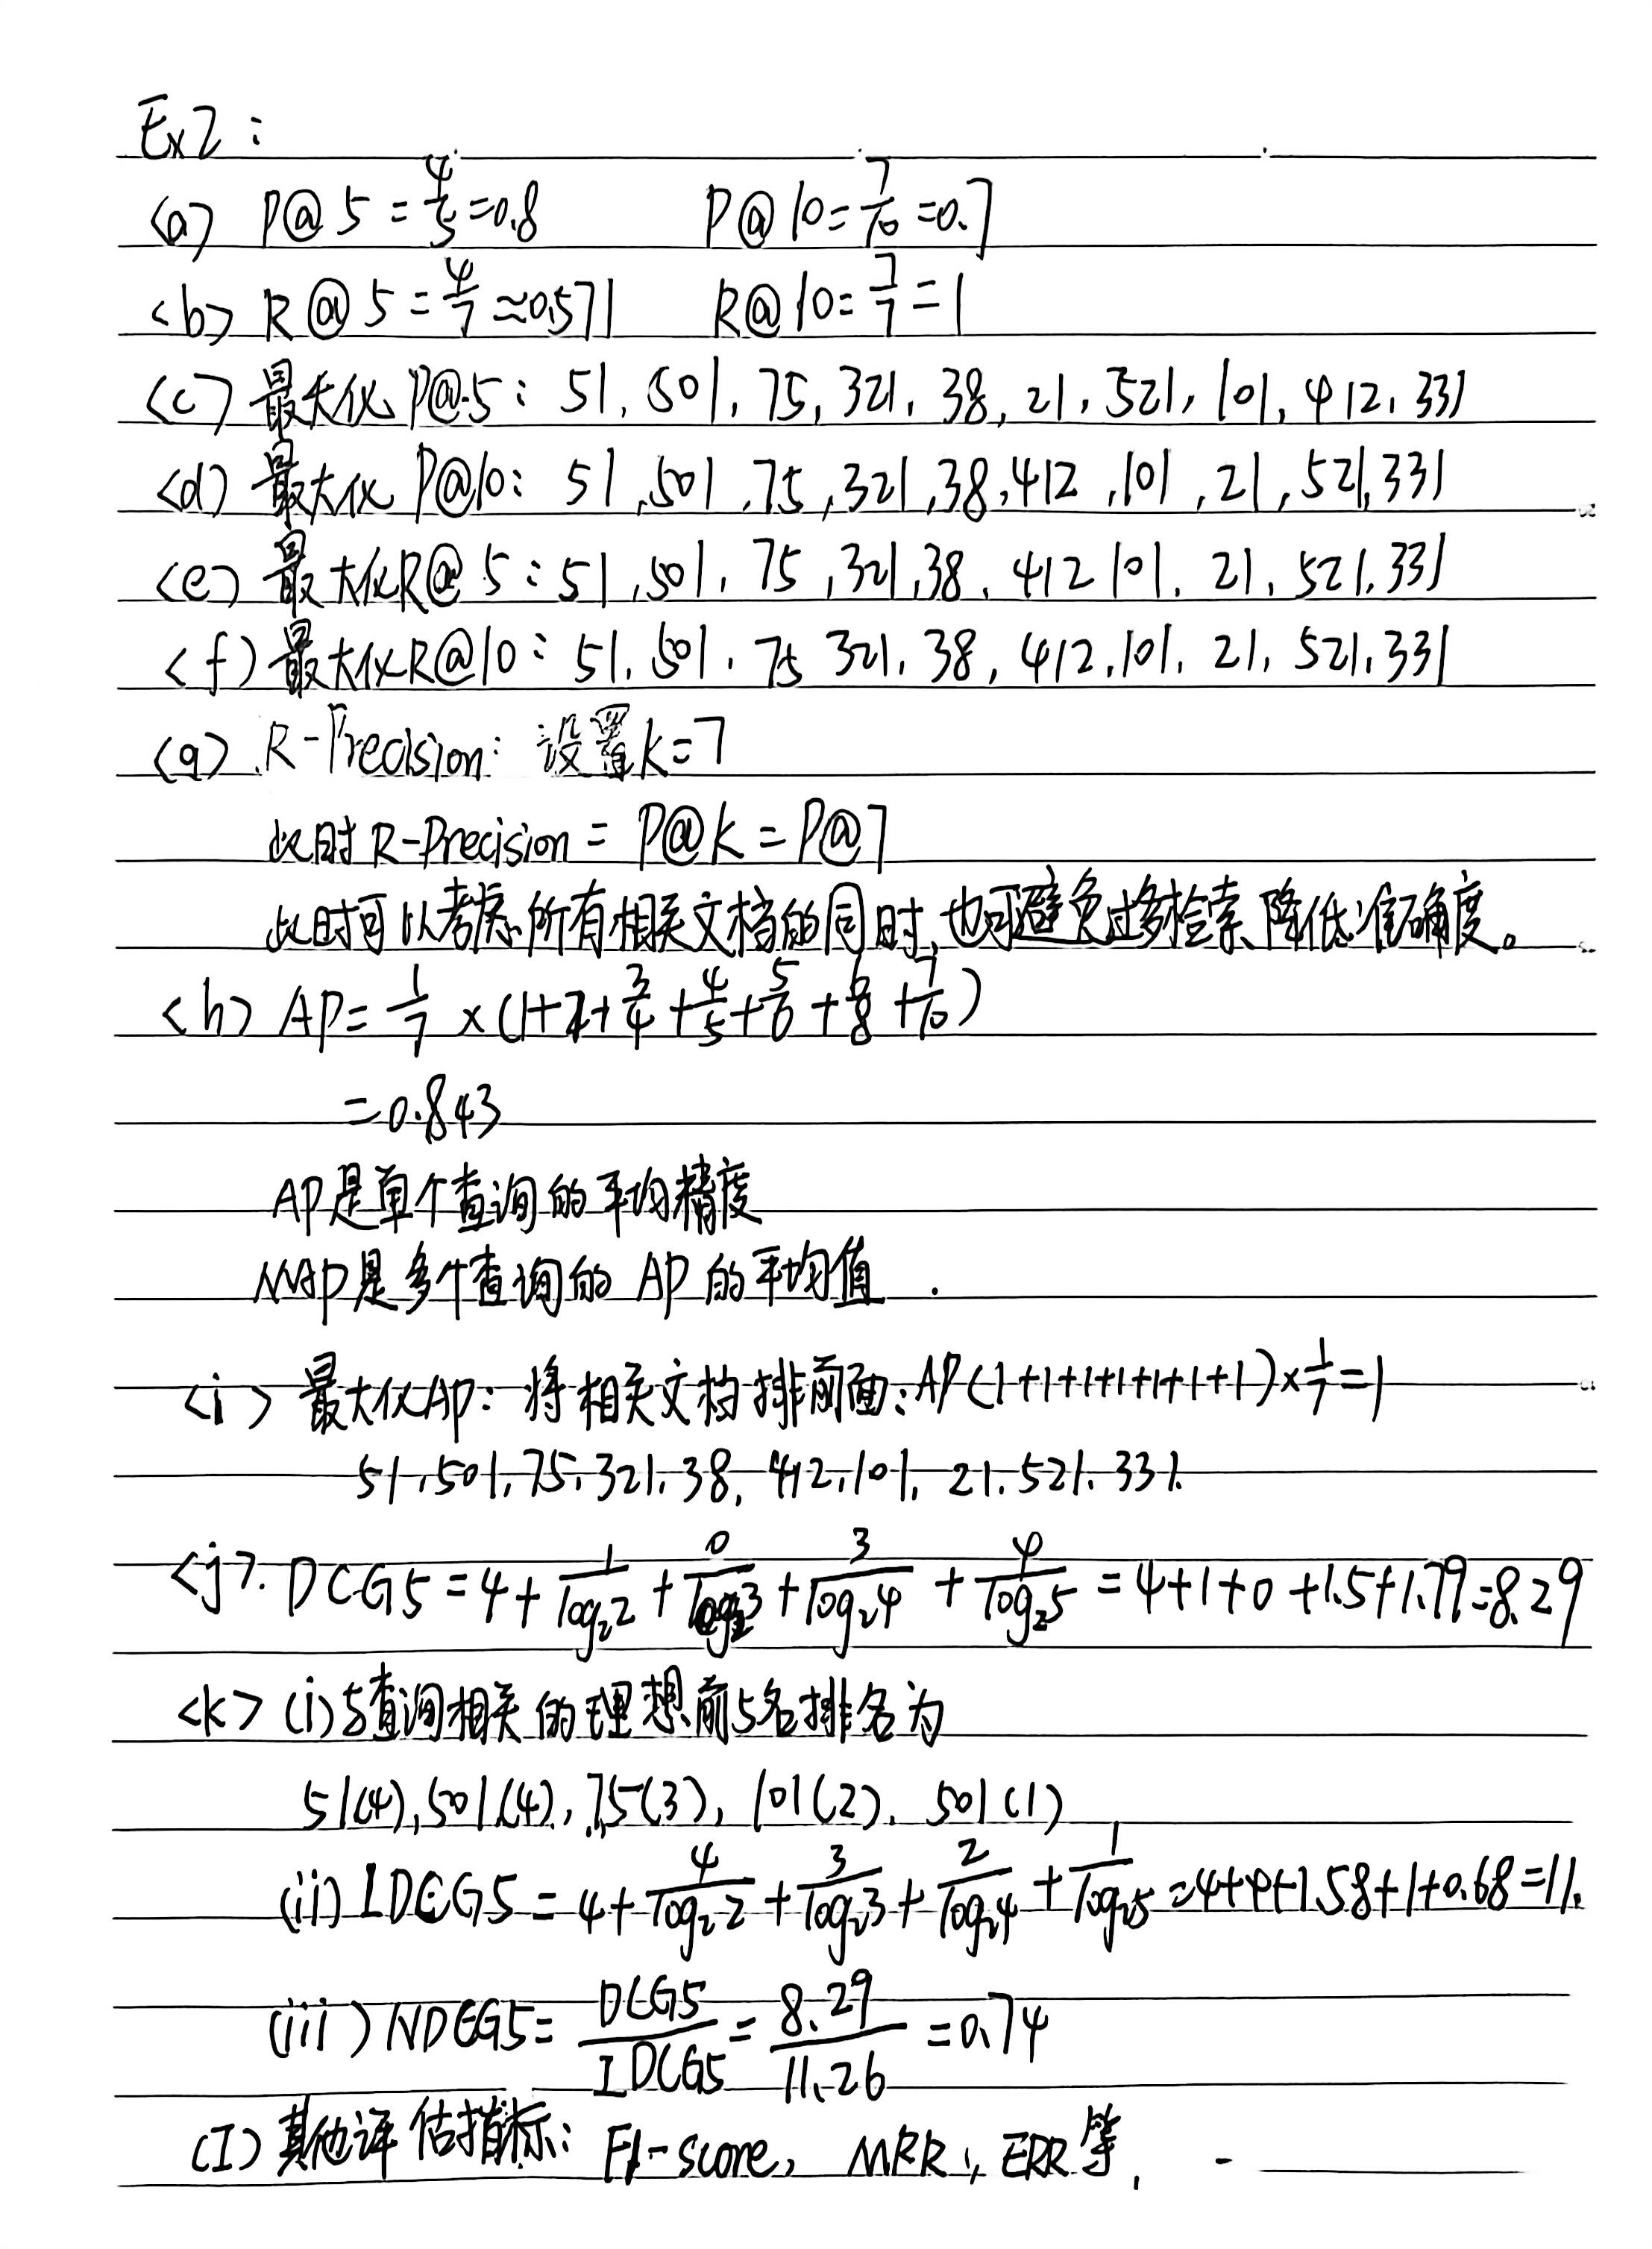
\includegraphics[width=\textwidth]{img/ex2_result.png}
    \caption{练习2计算过程}
    \label{fig:ex2_result}
\end{figure}

\section{练习3: 精度-召回率曲线}

精度-召回率（PR）曲线将精度表示为召回率的函数。通常，为评估集中的每个查询计算PR曲线，然后求平均。为简单起见，此问题的目标是为单个查询绘制PR曲线。绘制与练习2中排名相关的PR曲线（相同查询，相同结果）。（提示：您的PR曲线应该随着召回率水平的增加而始终下降。）


\begin{figure}[H]
    \centering
    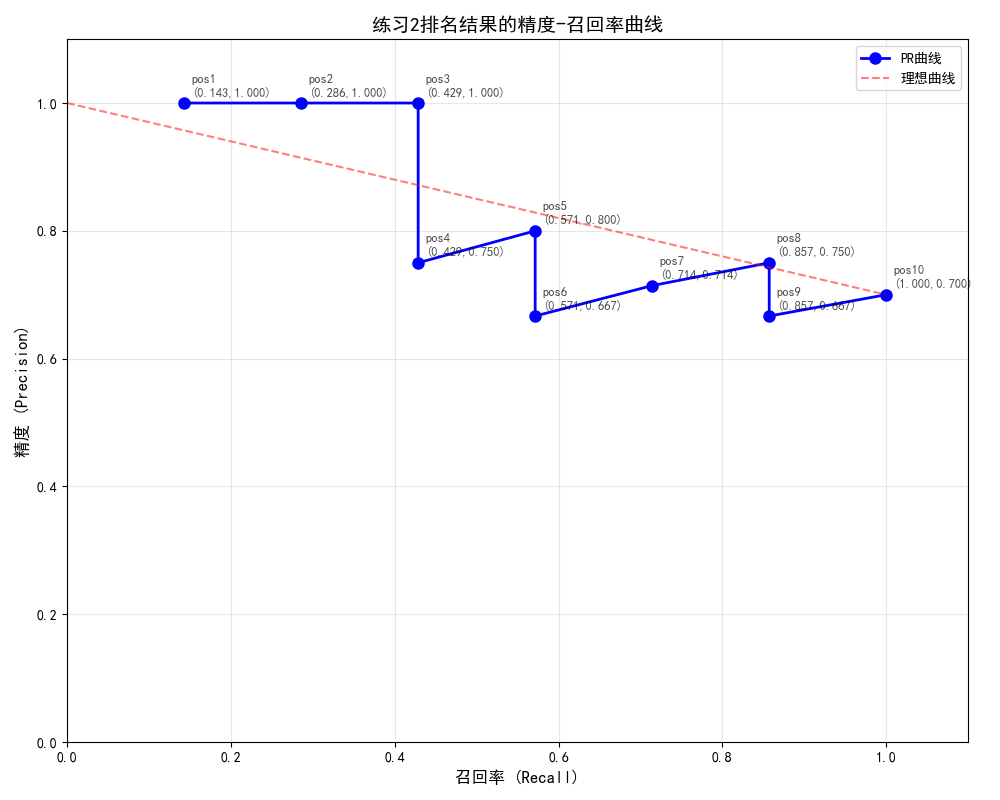
\includegraphics[width=\textwidth]{img/ex3_result.png}
    \caption{练习3结果}
    \label{fig:ex3_result}
\end{figure}

\section{练习4: 其他评估指标}

除了我们在讲座幻灯片中提到的指标外，是否还有其他评估指标可用于评估数据挖掘中特定任务的性能？这些任务是什么？如何计算这些评估指标？（提示：使用互联网查找您的答案。）

\subsection{分类任务评估指标}

\subsubsection{AUC-ROC (Area Under ROC Curve)}
\textbf{任务：} 二分类问题的性能评估

\textbf{计算方法：} ROC曲线下的面积。ROC曲线以假正例率(False Positive Rate)为x轴，真正例率(True Positive Rate)为y轴绘制。
\begin{align}
\text{TPR} &= \frac{\text{TP}}{\text{TP + FN}} \\
\text{FPR} &= \frac{\text{FP}}{\text{FP + TN}}
\end{align}

AUC-ROC值越接近1，分类器性能越好。

\subsubsection{AUC-PR (Area Under PR Curve)}
\textbf{任务：} 不平衡数据集的分类问题评估

\textbf{计算方法：} 精度-召回率曲线下的面积。相比AUC-ROC，AUC-PR在数据不平衡时更能反映模型的真实性能。

\subsubsection{F-beta Score}
\textbf{任务：} 需要在精度和召回率间进行加权的分类任务

\textbf{计算方法：}
$$F_\beta = (1+\beta^2) \times \frac{\text{precision} \times \text{recall}}{\beta^2 \times \text{precision} + \text{recall}}$$

其中$\beta > 1$更重视召回率，$\beta < 1$更重视精度。$F_1$是$\beta = 1$的特殊情况。

\subsection{回归任务评估指标}

\subsubsection{RMSE (Root Mean Square Error)}
\textbf{任务：} 回归预测任务

\textbf{计算方法：}
$$\text{RMSE} = \sqrt{\frac{1}{n}\sum_{i=1}^{n}(y_{\text{true},i} - y_{\text{pred},i})^2}$$

RMSE对大误差更敏感，适用于希望严格控制大误差的场景。

\subsubsection{MAE (Mean Absolute Error)}
\textbf{任务：} 回归预测任务

\textbf{计算方法：}
$$\text{MAE} = \frac{1}{n}\sum_{i=1}^{n}|y_{\text{true},i} - y_{\text{pred},i}|$$

MAE对异常值不敏感，提供误差的平均大小。

\subsubsection{MAPE (Mean Absolute Percentage Error)}
\textbf{任务：} 需要相对误差评估的回归任务

\textbf{计算方法：}
$$\text{MAPE} = \frac{1}{n}\sum_{i=1}^{n}\left|\frac{y_{\text{true},i} - y_{\text{pred},i}}{y_{\text{true},i}}\right| \times 100\%$$

\subsection{聚类任务评估指标}

\subsubsection{Silhouette Score}
\textbf{任务：} 无监督聚类质量评估

\textbf{计算方法：} 对于每个样本$i$，计算：
\begin{align}
a(i) &= \text{样本i与同簇其他样本的平均距离} \\
b(i) &= \text{样本i与最近邻簇样本的平均距离} \\
s(i) &= \frac{b(i) - a(i)}{\max\{a(i), b(i)\}}
\end{align}

轮廓系数为所有样本$s(i)$的平均值，取值范围[-1,1]，越接近1表示聚类效果越好。

\subsubsection{Adjusted Rand Index (ARI)}
\textbf{任务：} 有真实标签时的聚类结果评估

\textbf{计算方法：} 基于混淆矩阵，调整了随机分类的影响：
$$\text{ARI} = \frac{\text{RI} - \text{Expected RI}}{\text{max(RI)} - \text{Expected RI}}$$

取值范围[-1,1]，1表示完全匹配，0表示随机分类水平。

\subsubsection{Davies-Bouldin Index}
\textbf{任务：} 聚类紧密性和分离性评估

\textbf{计算方法：}
$$\text{DBI} = \frac{1}{k}\sum_{i=1}^{k}\max_{j \neq i}\left(\frac{\sigma_i + \sigma_j}{d(c_i, c_j)}\right)$$

其中$\sigma_i$是簇i的平均内部距离，$d(c_i, c_j)$是簇中心距离。值越小表示聚类效果越好。

\subsection{推荐系统评估指标}

\subsubsection{Hit Rate@K}
\textbf{任务：} 推荐系统命中率评估

\textbf{计算方法：}
$$\text{Hit Rate@K} = \frac{\text{前K个推荐中包含相关物品的用户数}}{\text{总用户数}}$$

\subsubsection{Coverage}
\textbf{任务：} 推荐系统多样性评估

\textbf{计算方法：}
$$\text{Coverage} = \frac{\text{被推荐的不同物品数量}}{\text{总物品数量}}$$

高覆盖率表示推荐系统能够推荐更多样化的物品。

\subsubsection{Novelty}
\textbf{任务：} 推荐新颖性评估

\textbf{计算方法：}
$$\text{Novelty} = -\frac{1}{|R|}\sum_{i \in R}\log_2 P(i)$$

其中$P(i)$是物品$i$在全体用户中的流行度，新颖性越高表示推荐了越多小众物品。

\subsection{信息检索特定指标}

\subsubsection{ERR (Expected Reciprocal Rank)}
\textbf{任务：} 考虑用户满意度的排序评估

\textbf{计算方法：}
$$\text{ERR} = \sum_{r=1}^{n} \frac{1}{r} \prod_{i=1}^{r-1} (1 - R_i) \times R_r$$

其中$R_i$是位置$i$处文档的相关性概率。

\subsubsection{bpref}
\textbf{任务：} 不完整相关性判断的检索评估

\textbf{计算方法：}
$$\text{bpref} = \frac{1}{R} \sum_{r} \left(1 - \frac{|\text{不相关文档排在相关文档r前}|}{R}\right)$$

适用于相关性判断不完整的情况。

\subsection{总结}

这些评估指标针对不同的数据挖掘任务和应用场景，能够更准确地评估模型在特定条件下的性能表现。选择合适的评估指标需要考虑任务类型、数据特征、业务需求等多个因素。在实际应用中，通常需要结合多个指标来全面评估模型性能。
\end{document}